
\documentclass[11pt]{article}
\usepackage[utf8]{inputenc}
\usepackage[english]{babel}
\usepackage[T1]{fontenc} % allows use of “<” etc in text
% \usepackage[scaled]{helvet} %use Helvetica for NASA stuff
% \renewcommand\familydefault{\sfdefault}  %non-default font stuff
% \usepackage[T1]{fontenc} %non-default font stuff
\usepackage{courier} %can do fixed-width with command \texttt{}
\usepackage{url} %allow file paths typesetting
\usepackage{amsmath}
\usepackage[]{amsthm} %lets us use \begin{proof}
\usepackage[]{amssymb} %gives us the character \varnothing
% \usepackage[citestyle=authoryear,bibstyle=numeric, natbib=true, backend=bibtex]{biblatex}
\usepackage[round,numbers,semicolon]{natbib} %round() in-text,numbers,;multiref
% \usepackage[super,numbers,comma]{natbib} %superscript in-text,numbers,;multiref
% \usepackage{apalike} %should use ampersand instead of 'and' for in-text citations
\bibliographystyle{abbrvnat}
% \bibliographystyle{plainnat}
% \bibliographystyle{apalike}
\setcitestyle{authoryear,open={(},close={)}} %in-text citations (Authors, Year)
% \setcitestyle{numbers} %in-text citations (number)
% \def\citeapos#1{\citeauthor{#1}'s (\citeyear{#1})}
\usepackage{amsfonts}
\usepackage{graphicx}
% \usepackage{fancyhdr} %fancy header for sections etc
% \usepackage{caption}
\usepackage[tableposition=top]{caption} % set table captions to the top
\captionsetup{labelsep=period} %do 'Figure 1. xxxx' instead of 'Figure 1: xxxx'
\captionsetup{font=footnotesize} %smaller caption font for all captions
% \captionsetup[figure]{font=footnotesize} %smaller caption font
% \usepackage{subcaption} 
% \usepackage{subfigure} 
% \usepackage{subfig} 
\usepackage[section]{placeins}
% \usepackage{xcolor}
\usepackage[table,xcdraw]{xcolor}
\usepackage{booktabs}
\usepackage[T1]{fontenc}  %NEW - T1 encoding. used for ditto marks
\usepackage[mathscr]{eucal} %mathcal font setting
\usepackage{lineno} %line numbers
% \linenumbers %toggle line numbers
\usepackage{hyperref} 
\hypersetup{colorlinks=true,linkcolor=black,citecolor=black,filecolor=black,urlcolor=blue} 
% \usepackage{titlesec} %to change section/subsection spacing
\usepackage[small]{titlesec} %to allow simple header size changes [big=default],[medium][small][tiny]
\usepackage{soul} %allows use of the ``\ul{}`` command for underlines that wrap around line breaks
\usepackage{hang} %hanging indents for text
\usepackage{wrapfig} %wrap text around a float/figure
% \pagestyle{fancy} %causes errors sometimes
\usepackage[final]{pdfpages}
\usepackage{enumerate} %allows you to choose enumerate style (i, I,etc)
% \usepackage{sectsty} %allows easy changes of section heading sizes
\usepackage{fancyvrb}  % allows you to insert literals/text files verbatim
\usepackage[titletoc,toc,title,page]{appendix} %numbered appendices 
\usepackage{bibentry} %allow in-text full citation 
\nobibliography*

%---- Fancy Label and formatting for literal file includes (fancyvrb)
% redefine \VerbatimInput
\RecustomVerbatimCommand{\VerbatimInput}{VerbatimInput}%
{fontsize=\footnotesize,
 %
 frame=lines,  % top and bottom rule only
 framesep=2em, % separation between frame and text
 rulecolor=\color{gray},
 %
 label=\fbox{\color{black}filename.txt},
 labelposition=topline,
 %
 commandchars=\|\(\), % escape character and argument delimiters for
                      % commands within the verbatim
 commentchar=*        % comment character
}
%---- Change the spacing between sections, paragraphs, etc
% \titlespacing*{\section}    %{<command>}{<left>}{<before-sep>}{<after-sep>} 
% {0pt}{0.0ex plus 0.1ex minus .1ex}{0.0ex plus .1ex}
% \titlespacing*{\subsection} %{<command>}{<left>}{<before-sep>}{<after-sep>}
% {0pt}{0.0ex plus 0.1ex minus .1ex}{0.0ex plus .1ex}
% \titlespacing*{\subsubsection} %{<command>}{<left>}{<before-sep>}{<after-sep>}
% {0pt}{0.0ex plus 0.1ex minus .1ex}{0.0ex plus .1ex}
% % \setlength{\parskip}{1em}	%lines to skip b/w paragraphs
% \setlength{\parskip}{0.0pt plus 1.0pt minus 1.0pt}	%lines to skip b/w paragraphs
\topmargin=-0.45in
\evensidemargin=0in
\oddsidemargin=0in
\textwidth=6.7in
\textheight=9.2in
\headsep=0.25in
% \topmargin=-0.45in
% \evensidemargin=0in
% \oddsidemargin=0in
% \textwidth=6.5in
% \textheight=9.0in
% \headsep=0.25in

%---- Change the section/subsection format size and style

%--[sectsty] (did not work well)
% \sectionfont{\large}%{\LARGE}
% \subsectionfont{\normalsize}%{\Large}
% \subsubsectionfont{\normalsize}%{\large}

% \title{Term Project Proposal:\\ Gas advection-diffusion in a fracture}
\author{John P. Ortiz}
\date\today
%This information doesn't actually show up on your document unless you use the maketitle command below

%Commands for ditto marks 
\newcommand*{\dittoclosing}{---''---}
\newcommand*{\dittostraight}{\textquotedbl} % available in T1 encoding
% \newcommand*{\dittostraight}{---\textquotedbl---} % available in T1 encoding

%Commands for text sub- and super-scripts
% \newcommand*{\sup}[1]{\ensuremath{^\textrm{{\scriptsize #1}}}} %didn't work
% \newcommand*{\sup}[1]{\textsuperscript{}} %didn't work
\newcommand\tsup[1]{\textsuperscript{#1}}
\newcommand*{\tsub}[1]{\textsubscript{{\scriptsize #1}}}
% \newcommand*{\tsub}[1]{\ensuremath{_\textrm{{\scriptsize #1}}}} %possibly doesn't work with sans serif font...
		
\DeclareMathOperator\erfc{erfc} %custom error function command

% %Table of contents modifications
% \addto\captionsenglish{
  % \renewcommand{\contentsname}%
    % {Table of Contents}%
% }
% }\renewcommand{\contentsname}{Table of Contents} %w/out Babel package
% \renewcommand\thechapter{\Roman{chapter}}
% \renewcommand\thesection{\arabic{section}} % “1 Section”
% \renewcommand\thesubsection{(\Alph{subsection})} % “(A) Subsection”
\renewcommand\thesection{\Alph{section}} % “A Section”
\renewcommand\thesubsection{\arabic{subsection}.} % “1. Subsection”
% \setcounter{secnumdepth}{0} % setting to 0 prints no numbers/letters/etc for sections/subsections
\setcounter{secnumdepth}{2} %sections are level 1, subsections are level 2

% For derivatives
\newcommand{\deriv}[1]{\frac{\mathrm{d}}{\mathrm{d}x} (#1)}

% For partial derivatives
\newcommand{\pderiv}[2]{\frac{\partial#1}{\partial#2}}
% \newcommand{\pderiv}[2]{\frac{\partial}{\partial #1} (#2)}

% Integral dx
\newcommand{\dx}{\mathrm{d}x}

% \renewcommand{\vec}[2]{\mathbf{#1}} %bold vectors instead of arrow

% \DeclareCiteCommand{\fullcite}
      % {\renewcommand{\finalnamedelim}
           % {\ifnum\value{liststop}>2 \finalandcomma\fi\addspace\&\space}
       % \begin{thebibliography}\thebibitem}
      % {\usedriver
         % {\DeclareNameAlias{sortname}{default}}
      % {\thefield{entrytype}}\finentry}
      % {\thebibitem}
      % {\end{thebibliography}}

\begin{document}
% \maketitle %This command prints the title based on information entered above

%------------------------------------------------------------- 
% 			 TITLE PAGE 
%------------------------------------------------------------- 
\begin{titlepage}
    \begin{center}
        \vspace*{4.5cm}
        % \Huge
        \LARGE
        \textbf{New Mexico Small Business Assistance}

        \textbf{(NMSBA)}
 
        \vspace{0.5cm}
        % \LARGE
        SlugTide How-to Guide 
 
        \vspace{4.5cm}

        % % \normalsize
        % \large
        % % \textbf{John P. Ortiz}
        % John P. Ortiz\tsup{1,3}, Dylan R. Harp\tsup{1}, Roger C. Wiens\tsup{2},
        % Harihar Rajaram\tsup{3}, Kevin W. Lewis\tsup{3}\\
        % \tsup{1}EES-16, \tsup{2}ISR-2, \tsup{3}Johns Hopkins University
% 
        % \vspace{1.5cm}

    \end{center}
        % \textbf{Abstract:}
        % \vspace{0.1cm}
% 
        % \normalsize 
        % The existence of methane on Mars is a topic of exceptional
        % a bit more about results.}
% 
        \vfill
 
        % \vspace{0.8cm}
        % \includegraphics[width=0.2\textwidth]{figs/jhu-academic_seal-bw}
        % \Large
        % EES-16
 
    % \end{center}
\end{titlepage}

\cleardoublepage
\pagenumbering{roman}
% %------------------------------------------------------------- 
% % 			 TITLE 
% %------------------------------------------------------------- 
% \noindent
% \begin{centering}
    % \textbf{NMSBA: Earth tide analysis writeup}
    % % \vspace{1cm}
% \end{centering}

\tableofcontents
  % \listoffigures
  % \listoftables

% \begin{appendix}
% \end{appendix}

\newpage




% \pagenumbering{roman}
\pagenumbering{arabic}

%------------------------------------------------------------- 
% 			 NOTE 
%------------------------------------------------------------- 
\section{Note}

Work in this document was performed using a local Mac version of MATLAB.  It
goes through several a couple examples of the \textsc{SlugTide} workflow with base path,
\texttt{<SlugTide>}, which represents the following path: 

    \path{/Users/jportiz/Documents/research/nmsba/SlugTide-copy/}


% %------------------------------------------------------------- 
% % 			 OUTLINE
% %------------------------------------------------------------- 
% \section{Outline}


%------------------------------------------------------------- 
% 			 EXAMPLE 1 – Xue2013 
%------------------------------------------------------------- 

\section{Example 1: Xue et al., 2013}

Based on data from the \citet{Xue2013} paper:

\vspace{0.5cm}
\bibentry{Xue2013}


%------------------------------------------------------------- 
% 			(1) Create working SlugTide directory 
%------------------------------------------------------------- 
\subsection{Create the working SlugTide directory}

Create the folder \texttt{Xue2013\_Example} with all thirteen (13) MATLAB
files. This will be the working directory and should contain:

\begin{itemize}
    \item \texttt{avg\_amp\_phase.m}             
    \item \texttt{BuildWell.m}
    \item \texttt{importfile.m}
    \item \texttt{InitiateWells.m}
    \item \texttt{LoadTides.m}
    \item \texttt{MasterWell.m}
    \item \texttt{nanmean.m}
    \item \texttt{nanstd.m}
    \item \texttt{PlotOriginalWL.m}
    \item \texttt{PlotWellResponse.m}
    \item \texttt{UserParam.m}
    \item \texttt{WaterResp\_general\_interp.m}
    \item \texttt{water\_respon\_time.m}
\end{itemize}

The functions \texttt{nanmean.m} and \texttt{nanstd.m} are included with this package as they are
not standard in every MATLAB installation but are used in the \textsc{SlugTide} codes.

You will also need to copy in the water level data file from this study
(\texttt{waterlevel.csv}). It can be downloaded from
\url{https://www.science.org/doi/suppl/10.1126/science.1237237/suppl_file/waterlevel.zip}.
The preview of the original downloaded data file is below:

\VerbatimInput[label=\fbox{\color{black}waterlevel.csv}]{/project/gas_seepage/jportiz/nmsba/Xue2013_Example/waterlevel-short.csv}


%------------------------------------------------------------- 
% 			(2) Prepare data files
%------------------------------------------------------------- 
\subsection{Prepare the data files}

Create individual .csv files for your data as columns of numeric data only. If
you have an unusual format, the easiest way to get started is to save the data
as two columns of text with the first column being days from 00:00:00 0/0/000
(MATLAB datenum convention) and the second being your water level depth. We
refer to this as the "Simple" format (Format code S). 

I chose to import the \texttt{waterlevel.csv} file into Excel and format it as
described above (2 columns; 00:00:00 0/0/0000). This is then saved as
\texttt{waterlevel\_preprocessed.csv}.

\begin{figure}[ht]
    \centering
    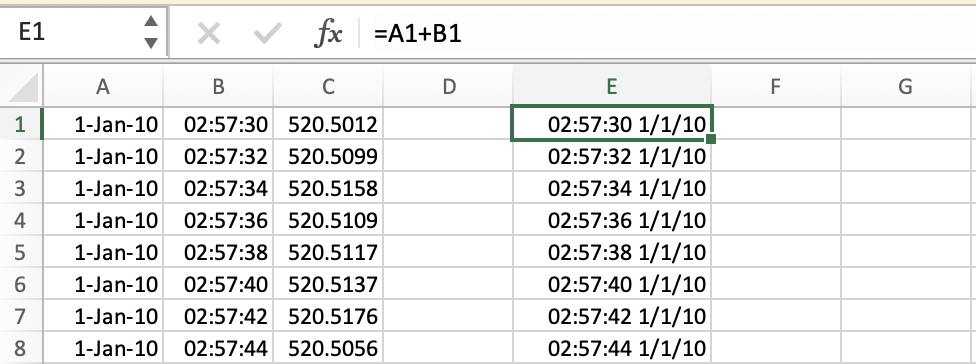
\includegraphics[width=0.5\textwidth]{../figs/howto/excel1.png}
    \caption{Example of how to combine the date and time in Excel. Excel will
    default to putting the date before the time, so you need to then choose
“Format > Cells” and select “Custom”. Then enter the following into the box:
\texttt{hh:mm:ss m/d/yy}.}
\end{figure}
\begin{figure}[ht]
    \centering
    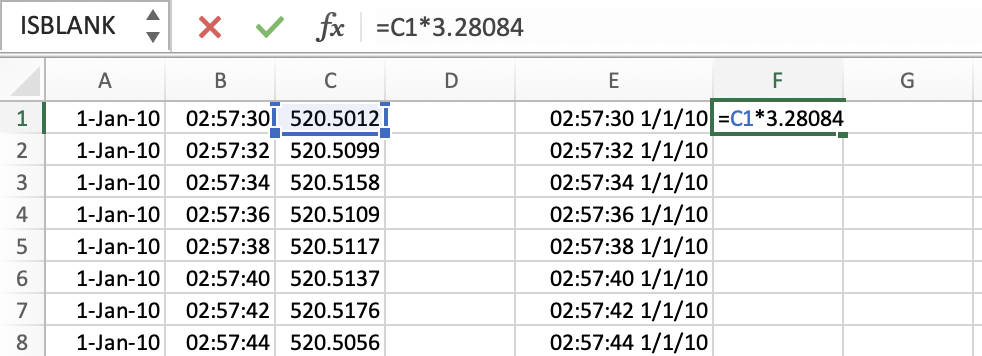
\includegraphics[width=0.5\textwidth]{../figs/howto/excel2.png}
    \caption{Convert the water level from meters to feet.}
\end{figure}
\begin{figure}[ht!]
    \centering
    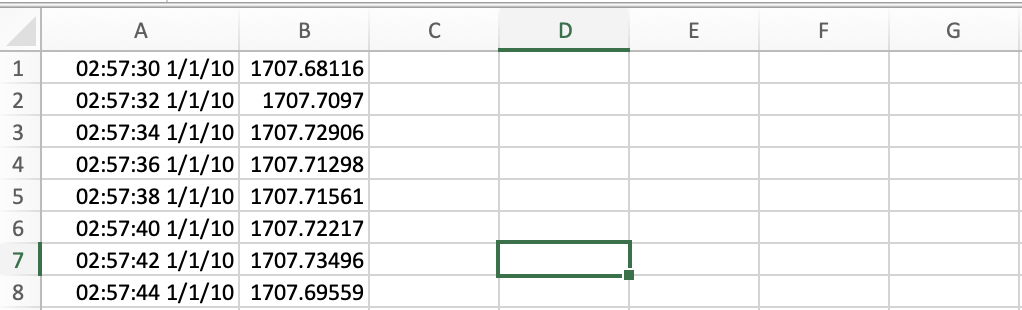
\includegraphics[width=0.5\textwidth]{../figs/howto/excel3.png}
    \caption{Resulting two column format that is then saved as a .csv file
    (\texttt{waterlevel\_preprocessed.csv}).}
\end{figure}

The resulting .csv file exported from Excel looks like this:

% \VerbatimInput[label=\fbox{\color{black}waterlevel_preprocessed.csv}]{/project/gas_seepage/jportiz/nmsba/Xue2013_Example/waterlevel\_preprocessed-short.csv}


\textbf{Note:} The original data file provided by the author has an issue where
there is a blank cell in the water level column when the time changes to
midnight (00:00:00). A hacky fix is to use excel to delete the rows where there
is a blank cell (the following website is a useful resource:
\url{https://www.howtoexcel.org/delete-blank-rows/}).

For this reason, I have 

\begin{figure}[ht!]
    \centering
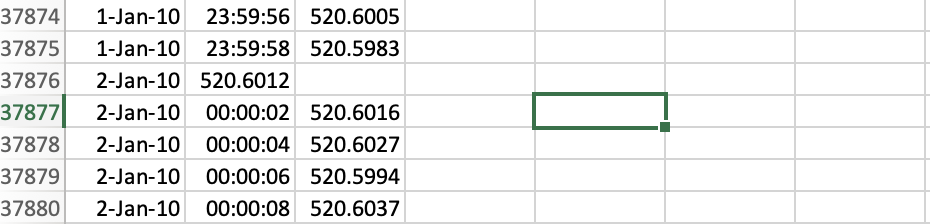
\includegraphics[width=0.5\textwidth]{../figs/howto/howto_excel-blank.png}
\caption{Issue with midnight data entries in the original data file.}
\end{figure}

%------------------------------------------------------------- 
% 			(3) Import data (importfile.m) 
%------------------------------------------------------------- 
\subsection{Import the data (\texttt{importfile.m})}

For this step, you can either: (a) preprocess your .csv file to match one of
the pre-defined formats or (b) edit the \texttt{importfile} function to better
match your data structure. 

The predefined formats are listed in the SlugTide documentation
(\textcolor{red}{Could include them eventually\dots}). 

The \texttt{importfile} function is called later in the \texttt{BuildWell.m}
script.  The \texttt{BuildWell.m} script can have multiple \texttt{importfile}
calls depending on the user-defined “format” of the data file you want to
import (e.g., `S', `A', `B', etc).


%------------------------------------------------------------- 
% 			(4) Create the TideSynth directory 
%------------------------------------------------------------- 
\subsection{Create the TideSynth directory}

Create a folder in your working directory called ``TideSynth'' (if it does not
already exist).

Create the synthetic tide files for the wells. Use SPOTL or another program
(see \ref{appendix:spotl} for details on how to do this). 
Each well processed needs to have its own synthetic tide file.

Save the synthetic tide files for all the wells in the dataset in a separate
folder ``TideSynth'' within the directory folder containing the .csv data files
and MATLAB codes.

For the well in \citet{Xue2013}, the relevant SPOTL input parameters are listed
below:
\begin{itemize}
    \item Lat/long: 31.1$^\circ$N, 103.7$^\circ$E
    \item Start date: 1/1/2010
    \item End date: 8/6/2011
    \item Time zone: ``Local Beijing time'' (China Standard Time [UTC-8])
\end{itemize}

Make sure you consider the time zone of your well data vs the time zone of the
SPOTL output (UTC).

Performed these calculations in:
\path{/home/jportiz/software/spotl/working/Xue2013}
\begin{itemize}
\item Ran \texttt{strains\_wfsd-1.scr}
\item Ran \texttt{compile\_areal\_strains.py}
\end{itemize}

%------------------------------------------------------------- 
% 			(5) Modify the parameters for the dataset (UserParam.m) 
%------------------------------------------------------------- 
\subsection{Modify the parameters for the dataset (\texttt{UserParam.m})}

\begin{itemize}
    \item Open UserParam.m and edit the parameters for the test being studied.
        Parameters from this file are used within later steps in the process to
        calculate and plot the tidal response. Updating the parameters in this
        part of the code will negate the necessity to edit some of the
        individual steps later in the process.  
    \item If there are earthquake occurrences in the data, see the note on
        Earthquakes in the introduction. Note: the earthquake mentioned in this
        study occurred in 2008, so the analysis here is looking at the
        permeability ``healing'' that occurred in the years after the
        earthquake. 
\end{itemize}

\textcolor{red}{Add more details to this eventually\dots}


%------------------------------------------------------------- 
% 			(6) Set up the initial structure of wells for the test (InitiateWells.m) 
%------------------------------------------------------------- 
\subsection{Set up the initial structure of wells for the test (\texttt{InitiateWells.m})}

The \texttt{InitiateWells.m} script sets up the initial structure for the
wells, which is input into building the Well structure for the dataset
(\texttt{BuildWell.m}). Initially in \texttt{InitiateWells.m}, there are inputs
for three wells, one per pre-defined format ('S', 'A' and 'B'). The user will
need to copy and paste the set of inputs by format 'S','A', or 'B' for the rest
of the wells in their dataset using these predetermined formats. Users can
change the parameters and add wells as needed within \texttt{InitiateWells.m}
for their test. If the user is adding different formats, they will need to
update \texttt{importfile.m} and \texttt{BuildWell.m} (steps 3 and 8,
respectively) in addition to \texttt{InitiateWells.m}.

\textcolor{red}{Add detailed instructions on this\dots}

\textcolor{red}{NOTE: for some reason, the script does not like a
\texttt{WellInitial(iWell).startrow} value of 1 or 2 for this
dataset\dots Using a higher value (e.g., 152) seems to help. (Try to
figure out why this is).}

\begin{itemize}
    \item depth to open interval: 800 m (2624.67 ft)
\end{itemize}

%------------------------------------------------------------- 
% 			(7) If using the quick method... 
%------------------------------------------------------------- 
\subsection{If using the quick method (utilizing \texttt{UserParam.m} and \texttt{InitiateWells.m}, following preprocessing), skip to Step 15: \texttt{MasterWell.m}}

Steps 8 through 14 \textcolor{red}{(CHECK THESE NUMBERS)} describe the process
of calculating and plotting the tidal response, with instructions on where to
edit if needed.

Exception: If the user has made changes to \texttt{InitiateWells}, be sure to make the
necessary corresponding changes as described above.


%------------------------------------------------------------- 
% 			(8) Load tide data (LoadTides.m) 
%------------------------------------------------------------- 
\subsection{Load tide data (\texttt{LoadTides.m})}

\textbf{Note:} Nothing is required from the user for this step.

This function loads the synthetic tides into the data structure within \texttt{BuildWell.m}

This code calls variables established in \texttt{UserParam.m}.

a.     Call the time interval of the synthetic tide data.

\begin{verbatim}
UserParam;
...
t=Well.t0_tide(i)+(0:length(y)-1)'*Tide_dt; 
\end{verbatim}

%------------------------------------------------------------- 
% 			(9) Build the Well structure for the dataset (Buildwell.m)
%------------------------------------------------------------- 
\subsection{Build the Well structure for the dataset (\texttt{Buildwell.m})}

This function calls variables established in \texttt{UserParam.m}.

This part of the code is written as a function that sets up the Well Structure
for the dataset through an \texttt{if elseif} loop using the formats as assigned to
the wells in \texttt{InitiateWells.m}.

\textcolor{red}{Add more info later\dots}


%------------------------------------------------------------- 
% 			(10) Plot original water level (PlotOriginalWL.m) 
%------------------------------------------------------------- 
\subsection{Plot original water level (\texttt{PlotOriginalWL.m})}

Plot the water level per well/port from the original data (not the interpolated
data).  This can be useful for identifying time periods with noisy data, and
for checking the times of earthquakes (if present).

This code calls variables established in \texttt{UserParam.m}.

\begin{enumerate}
    \item If there is an earthquake in the data, uncomment all earthquake
        related code in \texttt{PlotOriginalWL.m}, designated by:
\begin{verbatim}
    %%%% EQ.
\end{verbatim}

\item Establish time of EQ, if present in the data:
\begin{verbatim}
    EQ_t=datenum(EQtime)+cUTC; %%%%UTC %%%% EQ
\end{verbatim}

\item Establish time frame to plot (these variables are set in \texttt{UserParam.m}):
\begin{verbatim}
    xlim([datenum(PlotTime1) datenum(PlotTime2)])
\end{verbatim}

\item Plots are saved in both .pdf and .png file formats (see \ref{fig:origWLplot}).

\end{enumerate}


\begin{figure}[h]
    \centering
    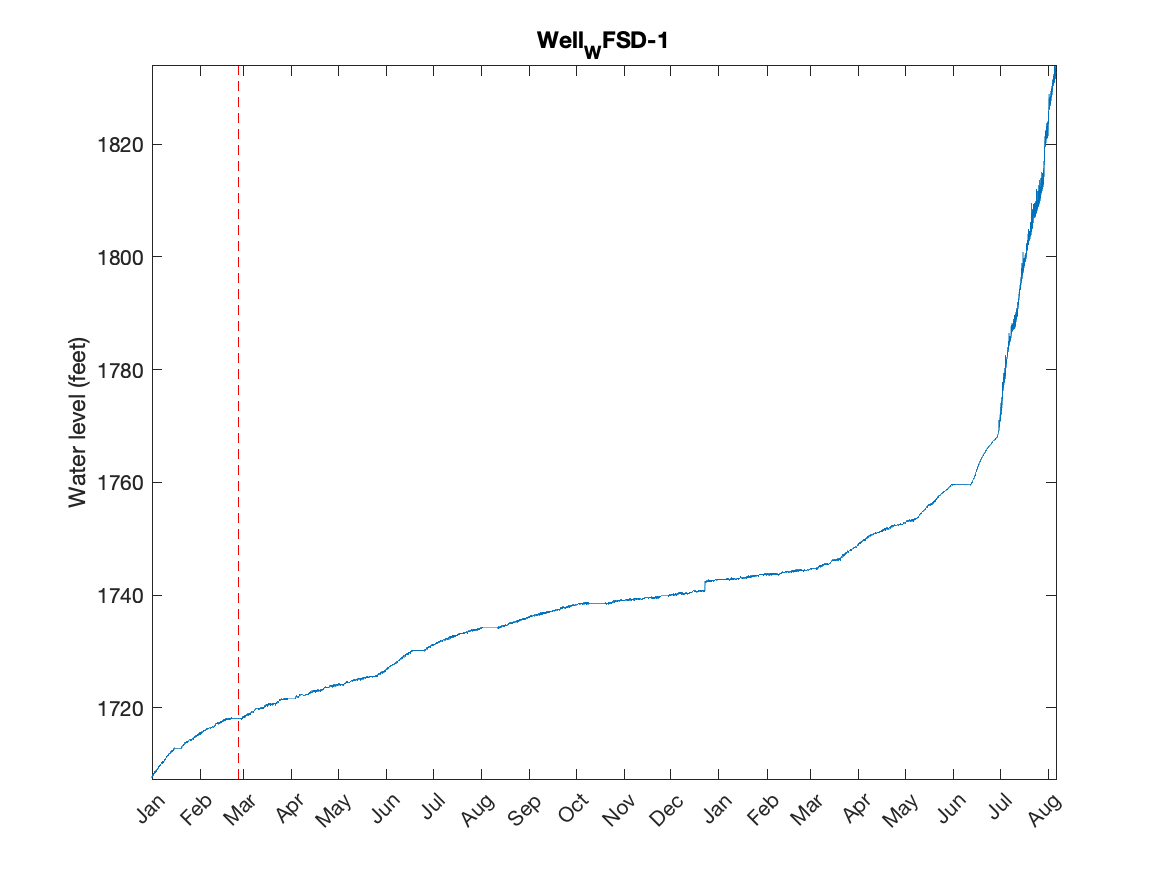
\includegraphics[width=1.0\textwidth]{../Well_WFSD-1_1_ori.png}
    \caption{Original water levels plot (before data interpolation);
    \texttt{Well\_WFSD-1\_1\_ori.pdf}.}
    \label{fig:origWLplot}
\end{figure}


%------------------------------------------------------------- 
% 			(11) Calculate the tidal components (Water_respon_time.m)
%------------------------------------------------------------- 
\subsection{Calculate the tidal components (\texttt{water\_respon\_time.m})}

This function performs the Fourier analysis and calculates the tidal components
called within \texttt{WaterResp\_general\_interp.m}.

The code calculates the response of the M2, S2, K1 and O1 tidal components.
Other tidal components may be added within this function, as needed for the
particular tidal study.

% \textcolor{red}{NOTE: This created an error when running the first time
% (``Error using \texttt{filtfilt}}. Expected input to be finite''). The error is
% traced to line 92 in WaterReesp\_general\_interp.}


%------------------------------------------------------------- 
% 			(12) Calculate the tidal response (WaterResp_general_interp.m)
%------------------------------------------------------------- 
\subsection{Calculate the tidal response (\texttt{WaterResp\_general\_interp.m})}

This code calls variables established in \texttt{UserParam.m}.
The sign convention for these calculations is extension positive.

%------------------------------------------------------------- 
% 			(13) Plot the Phase and Amplitude response (PlotWellResponse.m) 
%------------------------------------------------------------- 
\subsection{Plot the Phase and Amplitude response (\texttt{PlotWellResponse.m})}

This code calls variables established in \texttt{UserParam.m}.

\begin{figure}[h]
    \centering
    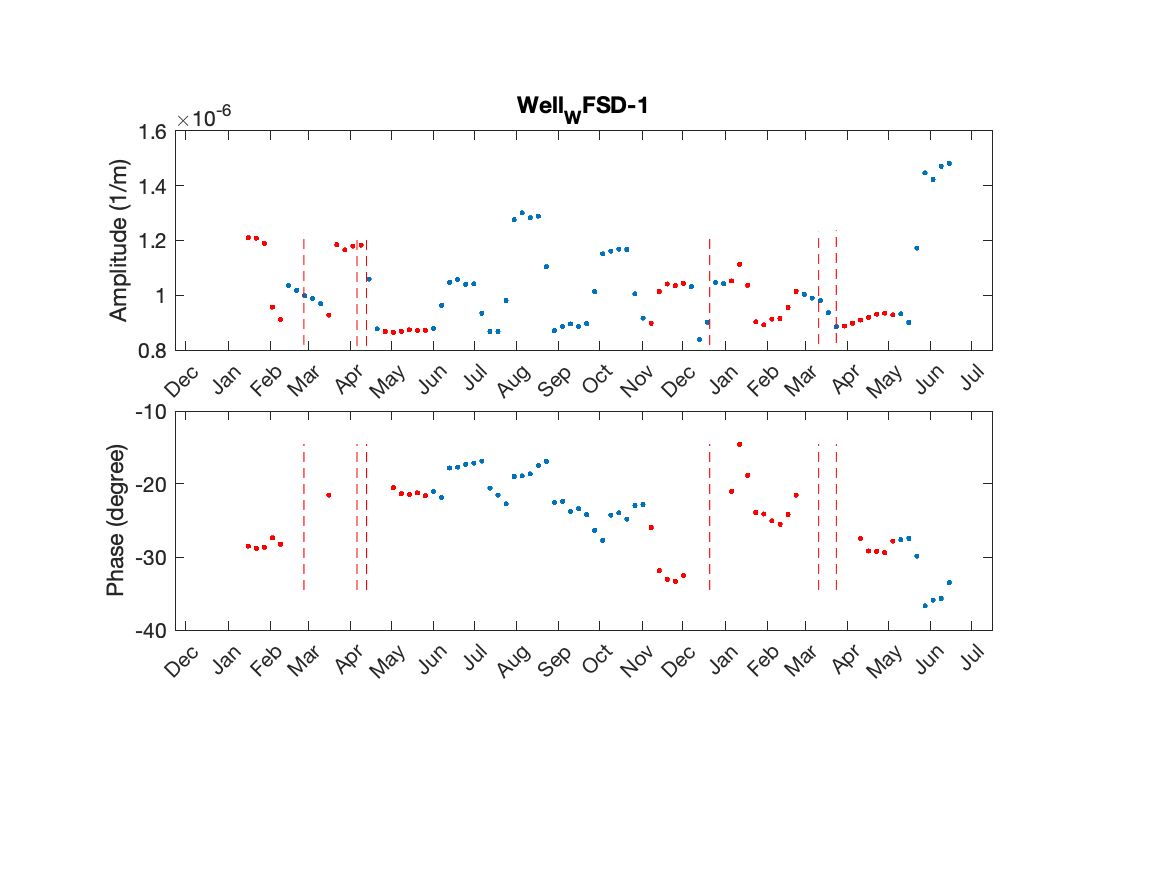
\includegraphics[width=1.0\textwidth]{../Well_WFSD-1_1_amp_pha.png}
    % 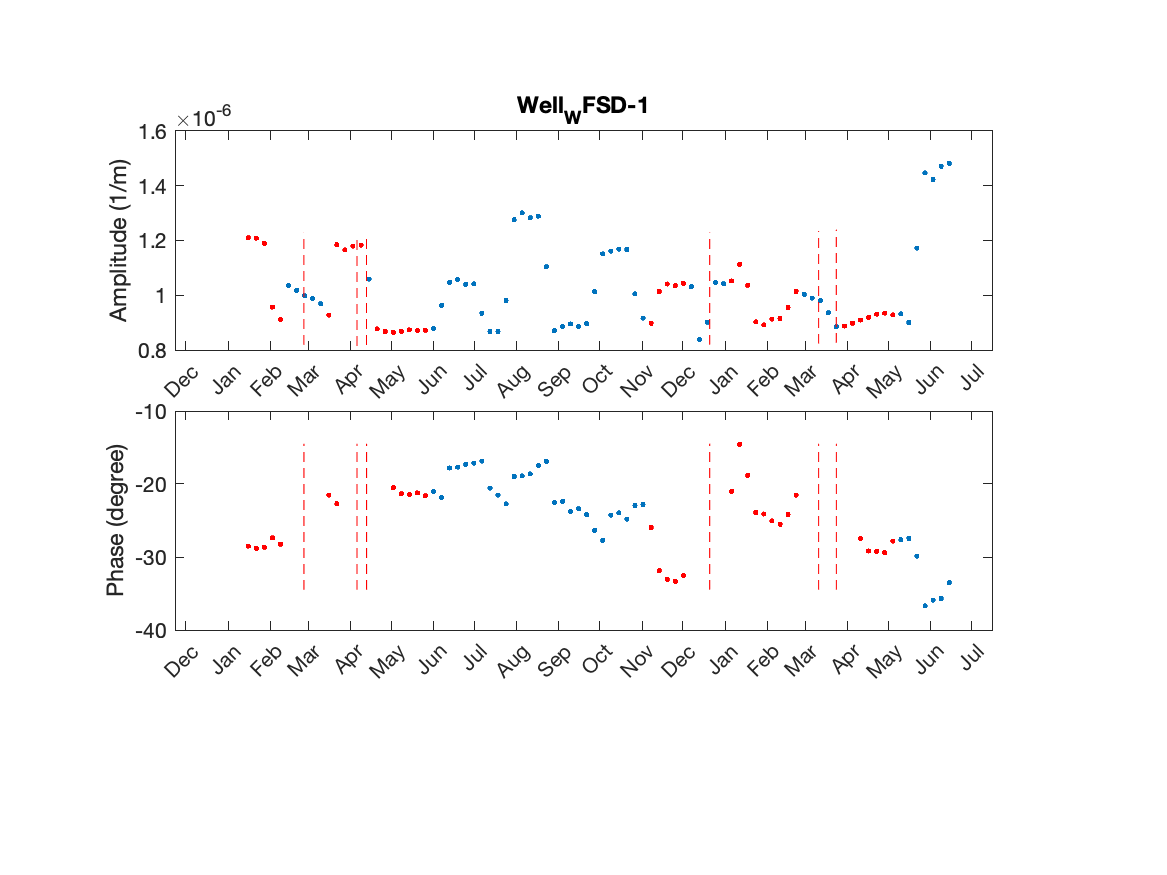
\includegraphics[width=1.0\textwidth]{{../Well_WFSD-1_1_amp_pha}.pdf}
    \caption{Phase response and amplitudes; \texttt{Well\_WFSD-1\_1\_amp\_pha.png}.}
    \label{fig:amp-pha-plot}
\end{figure}


%------------------------------------------------------------- 
% 			(14) Calculate and plot the average amplitude and phase for wells with multiple ports 
%------------------------------------------------------------- 
\subsection{Calculate and plot the average amplitude and phase for wells with
multiple ports over a specified time frame; \texttt{avg\_amp\_phase.m}}

This in an additional code that plots the average amplitude and phase response
in wells with depth of the ports for study of vertical control on tidal
response.
 
Plots are saved in both .pdf and .png file formats (e.g., \autoref{fig:avg-amp-pha-plot}).

\begin{figure}[h]
    \centering
    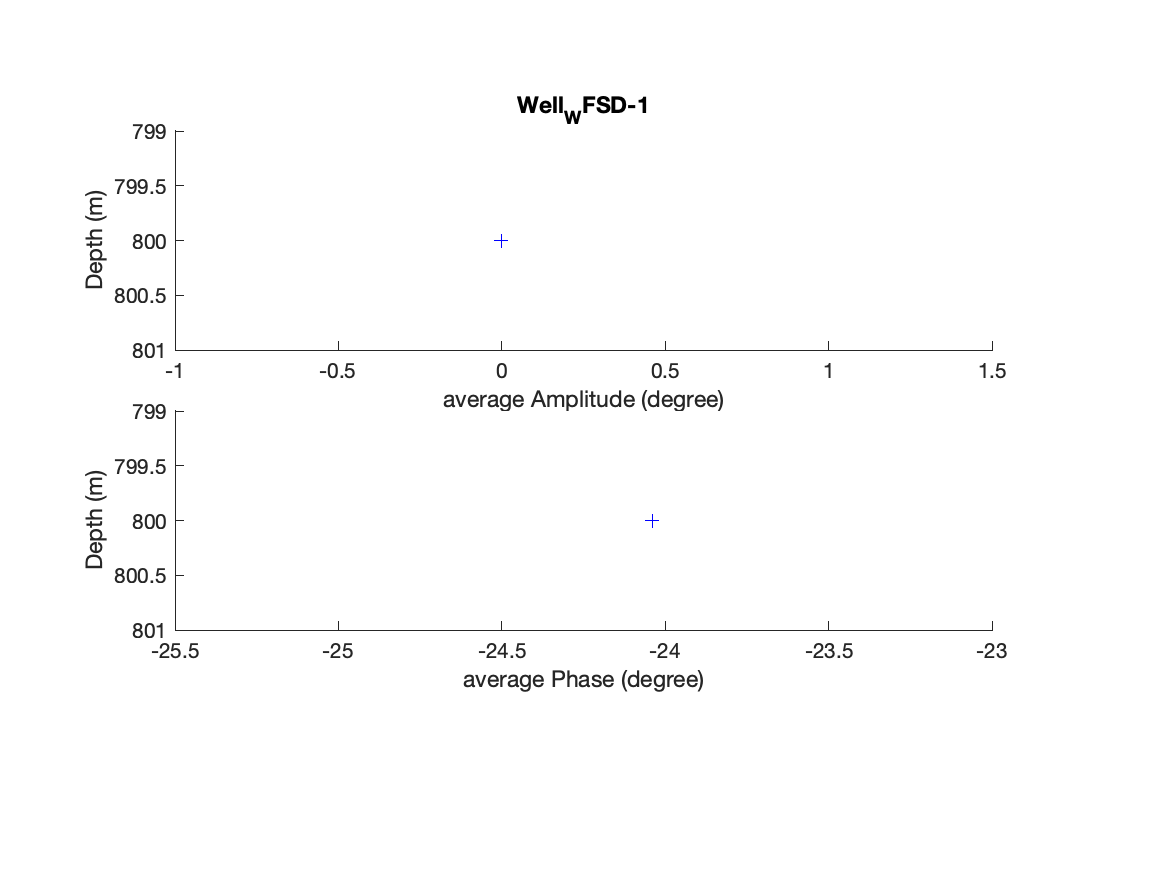
\includegraphics[width=1.0\textwidth]{../Well_WFSD-1_1_avg_amp_pha.png}
    % 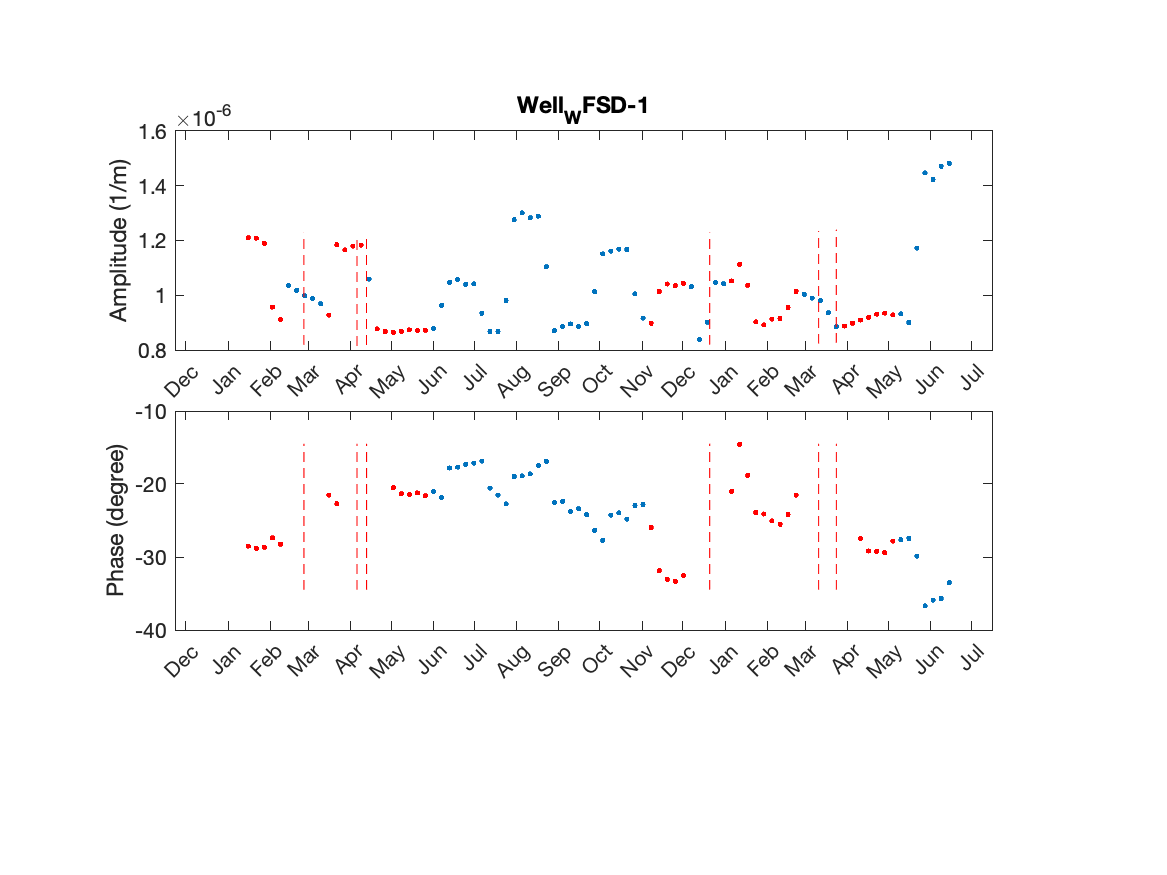
\includegraphics[width=1.0\textwidth]{{../Well_WFSD-1_1_amp_pha}.pdf}
    \caption{Average phase response and amplitudes; \texttt{Well\_WFSD-1\_1\_avg\_amp\_pha.png}.}
    \label{fig:avg-amp-pha-plot}
\end{figure}


%------------------------------------------------------------- 
% 			(15) Process the dataset; MasterWell.m 
%------------------------------------------------------------- 
\subsection{Process the dataset (\texttt{MasterWell.m})}

This code calls variables established in \texttt{UserParam.m} and
\texttt{InitiateWells.m}.




%------------------------------------------------------------- 
% 			 TIDAL ANALYSIS 
%------------------------------------------------------------- 
% \section{Tidal Analysis}


% \subsection{Prerequisites}

% \begin{itemize}
% \end{itemize}




% \path{<nmsba_path>/data/fuentes_arreazola2018/baro_efficiency_rahi.py} 
% \\

% \noindent\textit{Data Requirements:}
% \begin{itemize}
    % \item Water level data (well data)
    % \item Barometric pressure data
% \end{itemize}
% 


% \subsubsection{Tides and Areal Strain}
% 
% \path{<nmsba_path>/data/fuentes_arreazola2018/processed/tidal_frequencies.py}
% 
% In \citet{Fuentes-Arreazola2018}, amplitudes $A_{wk}$ and phases $\phi_{wk}$ of
% the filtered water-level were computed at their exact tidal frequencies from
% the regression coefficients obtained by fitting the water level data to a sum
% of sines and cosines functions using the “t\_tide” Matlab code. We have elected
% to use a version of “t\_tide” that has been converted to Python (“ttide\_py”;
% \url{https://github.com/moflaher/ttide_py.git}). Recall that the component
% frequencies $O_1$ and $M_2$ are often the only ones used for groundwater level
% response analysis. 
% 
% Amplitudes $A_{tk}$ and phases $\phi_{tk}$ of the calculated areal strain tide
% were also computed using the regression coefficients obtained by the “t\_tide”
% code, and \autoref{amplitude} and \autoref{phase_shift}. 
% Areal strain sensitivity was calculated using
% \autoref{areal_strain_sensitivity}. The phase shift will be utilized below in
% the calculation of transmissivity. 
% 
% \begin{equation}
    % A_{wk} = \sqrt{a_{wk}^2 + b_{wk}^2}
    % \label{amplitude}
% \end{equation}
% 
% \begin{equation}
    % \Phi_{wk} = \tan^{-1}\left({-\frac{b_{wk}}{a_{wk}}} \right)
    % \label{phase_shift}
% \end{equation}
% 
% 
% \begin{equation}
    % A_{sk} = \frac{A_{wk}}{A_{tk}} = - \frac{WL}{\epsilon_a} = \frac{A_{2k}(\tau_k,\theta)}{A_{hk}(\tau_k)}
    % \label{areal_strain_sensitivity}
% \end{equation}


% \VerbatimInput[label=\fbox{\color{black}arealStrainOutput}]{/project/gas_seepage/jportiz/nmsba/data/fuentes_arreazola2018/processed/arealStrainOutput}


% \path{<nmsba_path>/data/fuentes_arreazola2018/rock_properties/calc_properties.py}

% 
% \begin{table}[h!]
    % \centering
    % \caption{Well information. Coordinates are from the World Geodetic System,
    % WGS-84 datum, presented in decimal degrees. Adapted from
% \citet{Fuentes-Arreazola2018}.}
    % \begin{tabular}{cll}
        % \hline
        % \textbf{Well ID} & \textbf{Latitude} $(\theta)$ & \textbf{Longitude} $(\phi)$\\ \hline
        % PZ-01 & 32.4045 & -115.2343 
% \end{tabular}
% \label{well_info_table}
% \end{table} 
% 
% \begin{table}[h!]
    % \centering
    % \caption{Periods for the two tidal components of interest.}
    % \begin{tabular}{cl}
        % \hline
        % \textbf{Tidal Component} & \boldmath{$\tau$} [d] \\ \hline
        % $O_1$  & 1.0758 \\
        % $M_2$  & 0.5175
% \end{tabular}
% \label{tau_table}
% \end{table} 


% \begin{table}[h!]
% \centering
    % \caption{Adapted from Table 7 in \citet{Merritt2004}.\\ 
        % $\theta$ = latitude of observation point\\ 
        % $q$ = angular velocity of Earth relative to the mean sun (15$^\circ$
        % per mean solar hour)\\ 
        % $\phi_s(t)$ = longitude of mean sun (increasing
        % by 0.0411$^\circ$ per mean solar hour)\\ 
        % $\phi_m(t)$ = mean longitude of the moon (increasing by 0.549$^\circ$
        % per mean solar hour)\\ 
        % $\phi$ = longitude of observation point.}
% \begin{tabular}{clll}
% \hline
% \multicolumn{1}{l}{\textbf{Tidal Component}} & \boldmath{$b$}  & \boldmath{$f(\theta)$} & \boldmath{$\beta(\phi,f)$} \\ \hline
% $O_1$  & 0.377 & $\sin{\theta} \cos{\theta}$  & $qt+\phi_s(t)-2\phi_m(t)-169.8^\circ + \phi$  \\
% $M_2$  & 0.908 & $0.5 \cos^2{\theta}$          & $2(qt+\phi_s(t)-\phi_m(t)-79.8^\circ + \phi)$
% \end{tabular}
% \label{merritt_table}
% \end{table} 
% 

% \VerbatimInput[label=\fbox{\color{black}incompressibleRockPropertiesOutput}]{/project/gas_seepage/jportiz/nmsba/data/fuentes_arreazola2018/rock_properties/incompressibleRockPropertiesOutput}




%-------------------------------------------------------------
% 			 REFERENCES 
%------------------------------------------------------------- 
\clearpage
\hypersetup{colorlinks=true,linkcolor=black,citecolor=black,filecolor=black,urlcolor=black} 
\bibliography{library}


\newpage

%------------------------------------------------------------- 
% 			    APPENDICES	
%------------------------------------------------------------- 
\renewcommand{\appendixpagename}{\centering Appendices} %adds an 'Appendices' title
\begin{appendices}
\setcounter{secnumdepth}{1} %section numbering for rest of document was off (0)
\hypersetup{colorlinks=true,linkcolor=black,citecolor=black,filecolor=black,urlcolor=blue} 

%------------------------------------------------------------- 
% 			    APPENDIX A: SPOTL	
%------------------------------------------------------------- 
\section{SPOTL}
\label{appendix:spotl}

\noindent\textbf{Use:} Used for calculating theoretical areal strain.

\noindent\textbf{Source:} \textsc{SPOTL} source code can be downloaded for free at
\url{https://igppweb.ucsd.edu/\~agnew/Spotl/spotlmain.html}.

\noindent\textbf{License:} All the code is freely available (in both the monetary and
open-source usages of "free"). Additional discussion is included in the
distribution. Use of the code should be cited as \citep{Agnew2012}.
\\ \\ 

I had to modify a few lines of the Makefile and other scripts in order to get
it to compile correctly on my machine. I used
the \textsc{gfortran} compiler on Linux.  

We are interested in areal strain (or volumetric strain) but \textsc{ERTID}
does not provide it directly. To retrieve it, you just need to compute the
horizontal strain in two perpendicular directions (e.g., azimuth $0^\circ$ and
$90^\circ$, as below) and sum up the quantities. The included script produces
two output files, “th0” and “th90”, with these two strain time series.


\VerbatimInput[label=\fbox{\color{black}SPOTL/ERTID Script}]{/home/jportiz/software/spotl/working/example_fuentes/strains.scr}



% \clearpage
% %------------------------------------------------------------- 
% % 			    APPENDIX B: SLUGTIDE 
% %------------------------------------------------------------- 
% \section{SlugTide}
% \label{appendix:slugtide}
% 
% \noindent\textbf{Use:} Collection of \textsc{MATLAB} scripts for processing
% data and analyzing tidal responses from water well data. 
% 
% \noindent\textbf{Source:} \textsc{SlugTide} code can be downloaded at 
% \url{https://websites.pmc.ucsc.edu/~seisweb/SlugTide/}.
% 
% \noindent\textbf{License:} The \textsc{SlugTide} code is freely available for academic and
% non-profit use. Use of the code can be cited as \citep{Xue2013}.
% \\ \\ 
% 

\end{appendices}

\end{document}



